\chapter{Architecture}
Nous allons maintenant passer à la description de l'architecture de notre système en commençant par pour vous présenter l’architecture logique, suivi de l'architecture physique. Nous terminerons par l'observation des lien entre les exigences requises par notre Robot avec cette architecture.

\section{Architecture Logique}
Dans ce diagramme \ref{fig:architectureLogique}, nous avons encapsuler les fonctions primaires de notre Robot. Nous avons choisi de définir 9 \emph{Sous-systèmes logique} avec, comme bloc principal le Robot Planteur.
\begin{figure}[!ht]
\centering
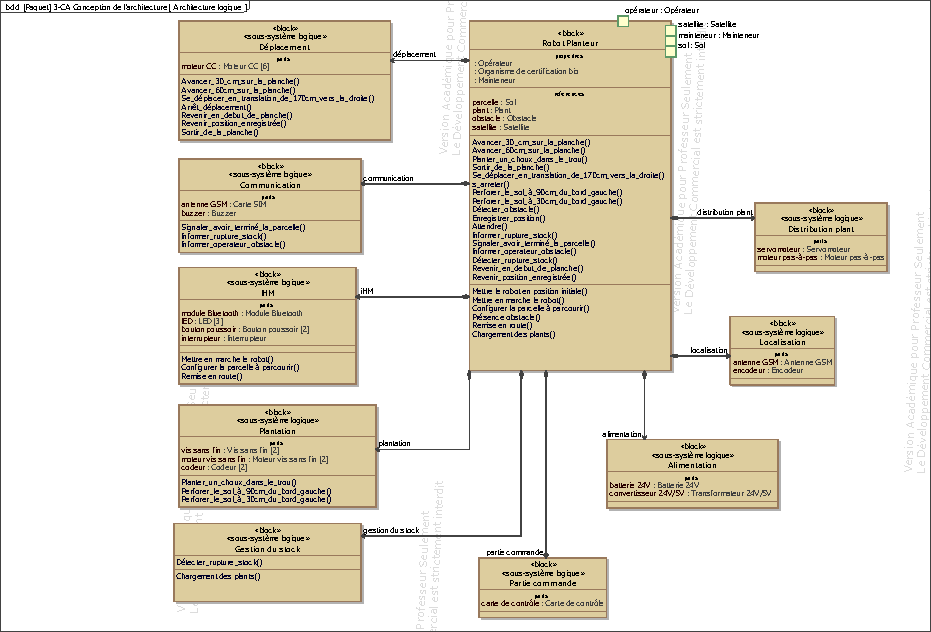
\includegraphics[width = \textwidth]{./III/images/SysML_Block_Definition_Diagram_3-CA_Conception_de_l_architecture_Architecture_logique.pdf}
\caption{Architecture Logique}\label{fig:architectureLogique}
\end{figure}
\subsection{Description des sous-systèmes logiques}
\paragraph*{Déplacement}
Ce \emph{Sous-système} doit permettre au robot d'avancer de manière précise sur la planche (30 cm ou 60 cm pour planter les différents plants), se sortir de la planche sans toucher et donc, en effectuant la translation aussi à disposition dans ce \emph{Sous-système}. Enfin, il doit permettre au robot d'être être capable de s'arrêter très rapidement et rester immobile après cet arrêt. 
\paragraph*{Communication}
Il permet d'informer l'opérateur si le robot se retrouve perturbé dans sa mission : un obstacle, une rupture de stock ou une fin du travail demandé. 
\paragraph*{IHM}
Le \emph{Sous-système} \textbf{Interface Homme Machine} doit permettre toute la configuration du système par l'opérateur. Il contient donc naturellement les fonctions de configuration et de mise en route. 
\paragraph*{Plantation}
Comme son nom l'indique, il doit permettre d'effectuer la fonction principale du robot. Toute la partie de perforation des sols est contenu dans ce \emph{Sous-système}. 
\paragraph*{Gestion du stock}
Il englobe tous l'ensemble de fonctions qui vont permettre de détecter les ruptures de stock en plants, et ce donc contient un ensemble de capteurs que nous détaillons en architecture physique (\ref{fig:architecturePhysique}).  
\paragraph*{Partie Commande}
Toute la gestion numérique permettant la commande du Robot seront contenu dans ce \emph{Sous-système}. Il convient donc d'utiliser des cartes électroniques programmable pour la réalisation de ces fonctions.
\paragraph*{Alimentation}
Ce \emph{Sous-système} doit permettre l'alimentation électrique de tout le robot. Il doit donc être suffisant puissant pour satisfaire en énergie toute les fonctions motrices du robot.
\paragraph*{Localisation}
Toute la gestion de l'emplacement du Robot sera contenu dans ce \emph{Sous-système}. Elle nécessitera un encodage pour permettre la communication des données avec plusieurs autres \emph{Sous-systèmes}.
\paragraph*{Distribution plant} 
Ce dernier \emph{Sous-système} va permettre l'approvisionnement en plants au bec du robot.  

\section{Architecture Physique}
Dans cette représentation \ref{fig:architecturePhysique}, nous avons établi le matériel qui sera utilisé pour remplir les fonctions logiques décrites plus tôt. Nous avons laissé libre choix sur les moteurs CC et les servomoteurs, sur les Vis et les moteurs associés, sur les parties communicantes, sur les batteries et transformateur et les composants de l'IHM. 
\begin{figure}[!ht]
\centering
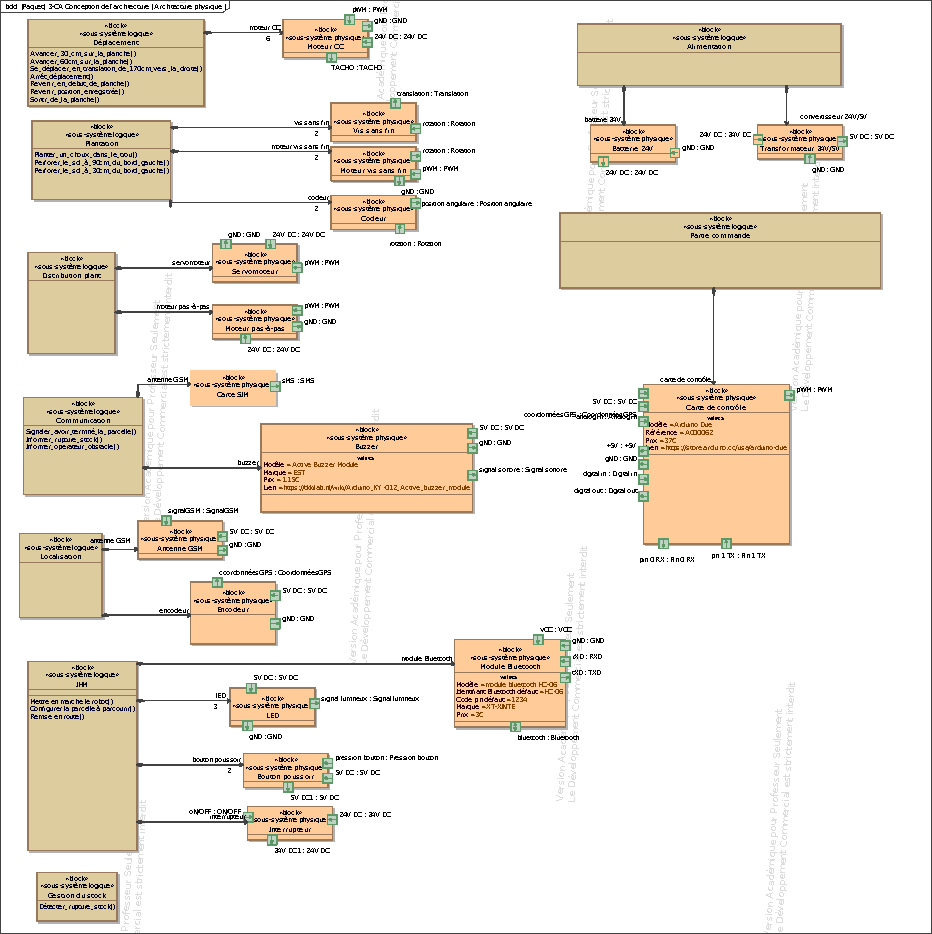
\includegraphics[width = \textwidth]{./III/images/SysML_Block_Definition_Diagram_3-CA_Conception_de_l_architecture_Architecture_physique.pdf}
\caption{Architecture Physique}\label{fig:architecturePhysique}
\end{figure}

\section{Traçabilité de la conception}
Chaque composant a, dans ce diagramme \ref{fig:tracabiliteConception}, été relié à un besoin. Nous remarquons, dans le cas de la \emph{carte de contrôle}, qu'elle est relié à tout les besoins : il s'agit d'une partie critique de notre système. La réalisation de cette partie devra demander beaucoup de précisions.
\begin{figure}[!ht]
\centering
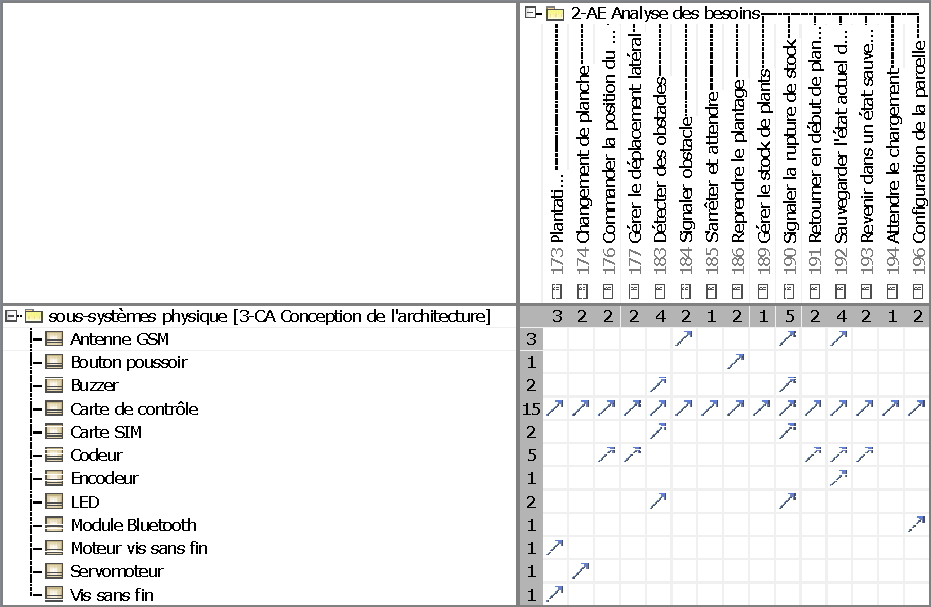
\includegraphics[width = \textwidth]{./III/images/Dependency_Matrix_3-CA_Conception_de_l_architecture_Tracabilite_conception.pdf}
\caption{Traçabilité de conception}\label{fig:tracabiliteConception}
\end{figure}
